\section{Verifying Context Switch Routine}
\label{sec:ctxswitch}

\indent
We apply our program logic to verify
that a context switch routine implemented in \sparc,
which is used to save the current task's context and
restore the new task's context, 
contextually refines the $\primsw{}$ primitive 
defined in \Sec{\ref{subsec:High-level Pseudo-SPARCv8 Language}}. 
\Fig{\ref{fig:The Structure of Context Switch Routine}}
shows the structure of the code.
\begin{center}
    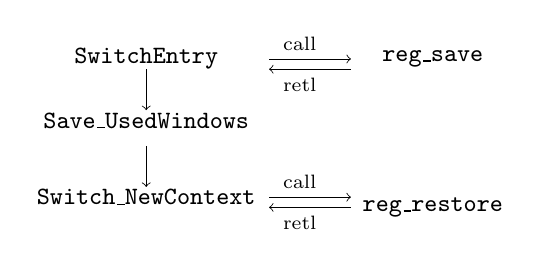
\begin{tikzpicture}[font=\small, line width=0.3pt, scale=1.3]
    \node(SwitchEntry) at (0, 2) {\texttt{SwitchEntry}};
    \node(call0) at (1.5, 2.15) {\scriptsize\text{call}};
    \draw[->] (1.2, 2) -- (2, 2);
    \node(retl0) at (1.5, 1.75) {\scriptsize\text{retl}};
    \draw[->] (2, 1.9) -- (1.2, 1.9);
    \draw[->] (0, 1.9) -- (0, 1.5);
    \node(regsave) at (2.8, 2) {\texttt{reg\_save}};

    \node(SaveUsedWindows) at (0, 1.4) {\texttt{Save\_UsedWindows}};
    \draw[->] (0, 1.15) -- (0, 0.75);

    \node(SwitchNewContext) at (0, 0.65) {\texttt{Switch\_NewContext}};
    \node(call1) at (1.5, 0.8) {\scriptsize\text{call}};
    \draw[->] (1.2, 0.65) -- (2, 0.65);
    \node(retl1) at (1.5, 0.4) {\scriptsize\text{retl}};
    \draw[->] (2, 0.55) -- (1.2, 0.55);
    \node(regrestore) at (2.8, 0.55) {\texttt{reg\_restore}};

    % \node(WindowOK) at (0, 1.4) {\texttt{Window\_OK}};
    % \draw[->] (-0.3, 1.25) -- (-1.6, 0.75);
    % \node(tcneqnull) at (-1.3, 1.2) {\tiny$t_c \neq \text{null}$};
    % \draw[->] (0.3, 1.25) -- (1.8, 0.5);
    % \node(tceqnull) at (1.3, 1.1) {\tiny$t_c = \text{null}$};

    % \node(regsave) at (-2, 0.6) {\texttt{reg\_save}};
    % \draw[->] (-2, 0.5) -- (-2, 0.1);
    % \node(SaveUsedWindows) at (-2, 0) {\texttt{Save\_UsedWindows}};
    % \draw[->] (-1.8, -0.15) -- (-0.5, -0.8);

    % \node(AdjustCWP) at (2, 0.3) {\texttt{Adjust\_CWP}};
    % \draw[->] (2, 0.2) -- (0.4, -0.8);
    % \node(SwitchNewContext) at (0, -0.9) {\texttt{Switch\_NewContext}};

    % \node(regrestore) at (2.8, -0.9) {\texttt{reg\_restore}};
    % \node(call) at (1.5, -0.7) {\tiny\text{call}};
    % \draw[->] (1.2, -0.85) -- (2, -0.85);
    % \node(retl) at (1.5, -1.1) {\tiny\text{retl}};
    % \draw[->] (2, -0.95) -- (1.2, -0.95);
\end{tikzpicture}
    \figurecaption{The Structure of Context Switch Routine}
	\label{fig:The Structure of Context Switch Routine}
\end{center}
\begin{itemize}
    \item \texttt{SwitchEntry}
    is the entry of the context switch routine. 
    It saves \localRN{} and \inRN{} registers of current
    window into stack (in memory), and call 
    \texttt{reg\_save} to save other registers into TCB.
    
    \item
    \texttt{Save\_UsedWindows} saves
	the register windows (except the current one)
    into the current task's stack in memory. 
    It checks whether the previous window is valid. 
    If it's valid, use the instruction $\crestore{}$ 
    to set the previous window as the current one, 
    and save its contents into stack (in memory), 
    then check the previous one continuously.

    \item     
    \texttt{Switch\_NewContext}
    restores the general registers from the new task's TCB 
    (by calling \texttt{reg\_restore})
    and its stack in memory 
    respectively. Then it sets the new task as
    the current one.
\end{itemize}

The main complexity of the verification lies in
the code manages the register windows.
To save all the used 
register windows, \texttt{Save\_UsedWindows}
repetitively restores the next window into general registers
(as the current window)
and then saves them into memory, until all the windows are saved.

\paragraph{\textbf{Specification.}}
Below we give the pre- and post-conditions
($\Apre$ and $\Apost$) of the verified module.
Each of them takes 6 arguments, 
the id of the current task $\ctid$, the id of the new 
task $\ntid$, the values $\env$ of general registers and all
other register windows, the new task's context $\nst$
that needs to be restored, and the thread local state 
of current task $\hthrdlocalst_c$ and the new task 
$\hthrdlocalst_n$.  
\[
    \small
    \begin{array}{l}
        \Apre(\ctid, \ntid, \env, \nst, \hthrdlocalst_c, \hthrdlocalst_n)
        \ \define \\
        \quad
        \begin{array}{l}
            \Env{\env} \sepstar
            (\relmsto{\TaskNew}{(\thrdid_n, 0)}) \sepstar 
            \metricAst{10} \sepstar \\
            \quad
            \RelCurT{\thrdid_c}{\notCare}{\env}{\hthrdlocalst_c} \sepstar 
            \RelRdyT{\thrdid_n}{\nst}{\hthrdlocalst_n} \sepstar 
            \safePrimAst{\, \primsw(\nil) \,}
        \end{array}
        \\
        \\[-8pt]
        \Apost(\thrdid_c, \thrdid_n, \env, \nst, \hthrdlocalst_c, \hthrdlocalst_n)
        \ \define \\ 
        \quad
        \begin{array}{l}
            \exists \, \env', \hthrdlocalst'. \, \Env{\env'} 
            \sepstar (\relmsto{\TaskNew}{(\thrdid_n, 0)}) 
            \sepstar \
            \\
            \quad
            (\RelCurT{\thrdid_n}{\nst}{\env'}{\hthrdlocalst'}
            \,\land\,\pEnv{\env'} = \nst) \sepstar 
            \\
            \qquad
            \RelRdyT{\thrdid_c}{\pEnv{\env}}{\hthrdlocalst_c} \sepstar 
            \safePrimAst{\, \primdone \,}
        \end{array}
    \end{array}
\]
In the specification,
we use $\Env{\env}$ to specify the values of
general registers and the register windows.
We describe the state
of the current task 
% (its TCB and stack in memory)
using $\RelCurT{\ctid}{\notCare}{\env}{\hthrdlocalst_c}$. 
It describes the memory of current task's TCB 
and stack for saving contexts in low-level, 
the thread local state $\hthrdlocalst_c$ in high-level, 
and the state relation between low- 
and high-level of the current thread $\ctid$.  
Similarly, $\RelRdyT{\ntid}{\nst}{\hthrdlocalst_n}$  
describes states of new task $\ntid$ in low- and high-level 
program and their relation. 
Here, we use $\nst$ to present the saved context 
of task $\ntid$. The memory location 
$\TaskNew$ records the identifier of the new task $\ntid$.  
And we use $\relmsto{\TaskNew}{(\ntid, 0)}$ to denote 
$\TaskNew$ saving $(\tid_n, 0)$ 
in both low- and high-level memory. 
\[
    \relmsto{\loc}{\val} \ \define \ 
    (\msto{\loc}{\val}) \sepstar (\hmsto{\loc}{\val})
\]

The precondition takes ten tokens ($\metricAst{10}$). 
As we have explained, verifying instruction \call{} 
and \jmp{} will consume a token. 
So, verifying calling function
\textsf{reg\_save} and \textsf{reg\_restore} will 
both consume a token. And \textsf{Save\_UsedWindows}, 
which checks each previous window 
and saves its contexts into memory until the invalid one, 
will execute at most eight times repetitively, 
because the upper bound of 
the number of windows is eight. 
So, ten tokens is sufficient. 

If we compare $\Apre$ and $\Apost$, we can see that
$\ntid$ becomes the current task
($\RelCurT{\ntid}{\nst}{\env'}{\hthrdlocalst'}$),
and its general registers and stack, specified by
$\Env{\env'}$, are loaded from the saved context
$\nst$ (\ie{} $\pEnv{\env'}\!=\!\nst$).
Here $\pEnv{\env'}$ refers to the part of the environment
that we want to save or restore as context.
Correspondingly, $\ctid$ becomes non-current-thread,
and part of its environment $\env$ at the entry of
the context switch is saved, as specified
$\RelRdyT{\ctid}{\pEnv{\env}}{\hthrdlocalst_c}$. 
The execution of $\primsw$ should be done in the final state. 
We use $\hthrdlocalst'$ to represent the thread local 
state of $\ntid$ instead of $\hthrdlocalst_n$ in final state, 
because the execution of $\primsw$ will modify the program counters 
in $\hthrdlocalst_n$. 